\section{Preliminary Results}
\label{sec-results}

As mentioned previously, we have performed a detailed analysis of 89~million
scan results collected from 139~smartphones over 5~months in order to
validate the usefulness of these measurements already being collected by
smartphones~\cite{conext14-pocketsniffer}. Encouraged by these results, we
have built a prototype \PS{} system including both an Android smartphone app
and adaptive AP. Because we have already explored asynchronous analyses that
can be performed using scan results, our preliminary results below focus on
what additional offline analyses can be done with more detailed channel
utilization information (\S\ref{subsec-rogue}) and on a basic form of online
channel adaptation (\S\ref{subsec-channel}).

To collect detailed channel utilization information, Wifi cards need to be
put in monitor mode so that every packet is delivered to upper layer---not
just ones addressed to the client. Unfortunately, few smartphone Wifi
chipsets currently support this feature out of the box\footnote{In some cases
monitor mode support can be achieved by modifying the firmware or device
driver~\cite{bcmon}.}, a challenge we return to in
Section~\ref{sec-challenges}. As a workaround allowing us to explore the
potential inclusion of this feature on next-generation smartphones, we
equipped several Galaxy Nexus~\cite{galaxynexus} smartphones with external
Wifi dongles including chipsets supporting monitor mode.
Table~\ref{tab:dongle} describes the Wifi dongle used in our experiments.

\begin{table}[t!]
  \centering
  {\small
  \begin{tabular}{ll}
    \toprule
    \textbf{Model} & ALFA Network AWUS036H \\
    \textbf{Chipset} & RTL8187L \\
    \textbf{Connector} & $1\times2.4$GHz SMA \\
    \textbf{Antenna} & 2.5dBi rubber duck \\
    \textbf{Wifi Support} & 802.11b/g \\
    \bottomrule
  \end{tabular}
}
  \caption{\textbf{Wifi dongle specification.}}
  \label{tab:dongle}
  \vspace*{-0.1in}
\end{table}


\subsection{Rogue Access Points}
\label{subsec-rogue}

Rogue APs (RAPs) are unauthorized APs deployed in areas designed to be
covered by existing enterprise wireless networks. RAPs are of concern to
network administrators both for security reasons and due to the unwanted
interference they may cause by competing with the official network for
spectrum resources. However, RAPs may be set up by users that feel
poorly-served by the official wireless network and if properly configured
they may not cause harmful interference. And realistically, our typical
campus network consisting of several thousand APs also contains hundreds of
RAPs, many more than available IT staff can deal with. A system like
\PS{} provides the ability to determine the impact of RAPs on clients'
network performance, allowing administrators to prioritize those that are
actually causing problems and ignore those that may be filling coverage
holes. To investigate the impact of RAPs, network administrators would
establish a \PS{} query asking devices to record short ($\sim$1~s) full packet
traces after scan results indicated the presence of a previously-identified
RAP.

Our department contains several RAPs. To investigate their impact, we
deployed 6~\PS{} devices: three were deployed statically in public areas,
with the remaining three carried by investigators for several hours each day.
All devices were put in continuous monitor mode in order to capture all
packet traffic, thus providing a superset of the data that would be provided
by actual \PS{} clients. In total, 38 device-hours worth of data containing
37~M packets were recovered. We first inspect beacon frames to identify APs.
Then we exclude campus APs and temporary hotspots with less than 1000~beacon
frames. 56~RAPs were detected in this way. For each RAP, we calculate the
total traffic volume (both down and up link) by summing up the length of all
data frames. Figure~\ref{fig:rap} shows 15 RAPs with most traffic, as well as
the number of devices that ever exchange data frames with them.

Among these 15~RAPs \texttt{AP1}~and~\texttt{AP2} are both operated by one of the
coauthors. \texttt{AP1} is unsecured which likely accounts for its higher
traffic volume and larger number of users, as it is available to users that
may not be able to authenticate to the campus network. \texttt{AP2} is
secured and only used by students in a particular room, and the large amount
of traffic it is serving might indicate a place where the campus network's
coverage could be improved. Other RAPs, such as \texttt{Parkhaven-Olewnik}
and \texttt{26capemay}, also generated large traffic volume yet all of them
are with one device, indicating personal RAPs that are secured and only used
by the owner.

\newpage

\begin{figure}[t]
  \centering
  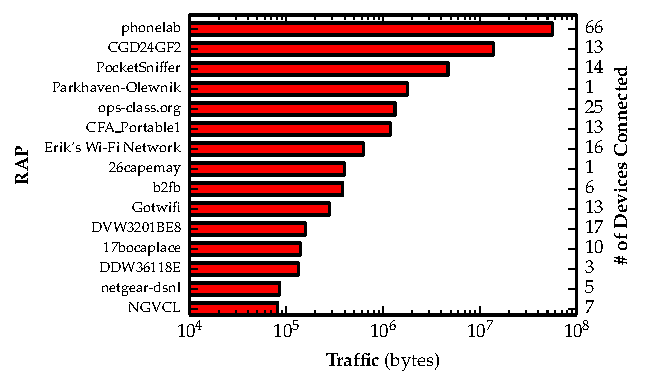
\includegraphics[width=\columnwidth]{./figures/RAPTrafficGraph.pdf}
  \vspace*{-4mm}
  \caption{\textbf{Measured Bandwidth to Rogue APs.}}
  \label{fig:rap}
  \vspace{-3mm}
\end{figure}


\subsection{Channel Assignment}
\label{subsec-channel}

To demonstrate how \PS{} can enable realtime network adaptation to improve
the performance of nearby active clients, we ran an experiment using a
sniffer device and an adaptive AP. The AP periodically requests channel
measurements from all available channels from the sniffer and uses the data
to determine the least-congested channel.

The experiment is designed as follows. We first set up a constant
\texttt{iperf} UDP session between \PS{}-AP $AP$ and device $D_1$ on channel
$C_1$. Then another device $D_2$ starts jamming the channel using UDP traffic
to simulate a new and serious source of interference. However, because the AP
is periodically retrieving channel utilization statistics from the sniffer
device it can react to the interference by determining which other available
channel is the least congested. All of this happens without disturbing $D_1$, 
which continues transferring data. All devices in this experiment are using
802.11g at 2.4GHz band. In the particular run shown in Figure~\ref{fig:bw},
from 0--8.5~s $A$ and $D_1$ establish stable UDP traffic on channel 11.

When $D_2$ starts jamming the channel at 8.5~s the link bandwidth between $A$
and $D_1$ decreases and begins to fluctuate. At 75~s, when $A$ and $D_1$
switch to a less congested channel (1), the bandwidth resumes to the level
obtained before the interference began. The latency between the onset of the
interference and the channel switch is due to several factors, including the
time required for the AP to initiate measurements, for the device to perform
the measurements, and for the device to transmit measurements to the AP, all
of which can be easily reduced in future prototypes.

\begin{figure}[t]
  \centering
  \vspace*{-1.3mm}
  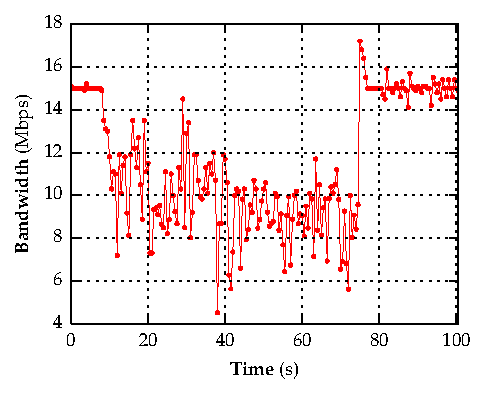
\includegraphics[width=\columnwidth]{./figures/ChannelBWGraph.pdf}
  \vspace*{-4mm}
  \caption{\textbf{Bandwidth between $A$ and $D_1$ after jamming (8.5~s) and
  channel switching (75~s).}}
  \label{fig:bw}
  \vspace*{-4mm}
\end{figure}
